\section{Introduction}
\label{sec:introduction}

LLM agents are becoming practical interfaces for complex enterprise procedure
automation: they plan, call tools, and modify shared services to complete
multi-step workplace tasks \citep{theagentcompany,selfevolving}. Their behavior
is governed by a static agent harness, including the software implementation,
system prompt, tools, environment interfaces, and fixed contexts supplied
before deployment \citep{coala}. Yet the operational knowledge needed in a
proprietary environment is intrinsically unforeseeable: under-documented APIs,
organization-specific policies, strict output conventions, abnormal service
states, and recovery paths often surface only during execution. In production,
designers cannot know in advance which hidden condition will cause the next
failure. Compounding this, unlike many coding or mathematical benchmarks where
broadly available knowledge combines with compilers, tests, exact answers, or
resettable sandboxes to provide cheap verification
\citep{swebench,mathdataset}, enterprise feedback depends on dedicated
proprietary environments and organization-specific outcomes, making evaluation
and diagnosis substantially more expensive \citep{theagentcompany}.

Long-term memory offers a training-free way to close this residual knowledge
gap without changing model parameters \citep{coala,memsurvey}. Episodic memory
preserves what happened in a particular rollout; semantic memory stores general
facts or concepts. Procedural memory, in contrast, captures how to act under
particular conditions
\citep{tulving1972,cohen1980,squire1992,anderson1993}. Its unit is not a
transcript or isolated statement but reusable guidance specifying when a
procedure applies, which actions and implementation details carry it out, what
can fail, and how to recover. Consequently, procedural memory requires
consolidation rather than naive accumulation: repeated successes should be
merged, contradictions resolved, and diagnosed failures incorporated as
missing preconditions or troubleshooting paths
\citep{automanual,awm,memp}. Without such consolidation, raw sessions accumulate
redundancy and noise without becoming accurate, robust knowledge that
generalizes across recurring task instances.


\begin{figure}[tb]
\centering
\begin{subfigure}[b]{0.56\linewidth}
  \centering
  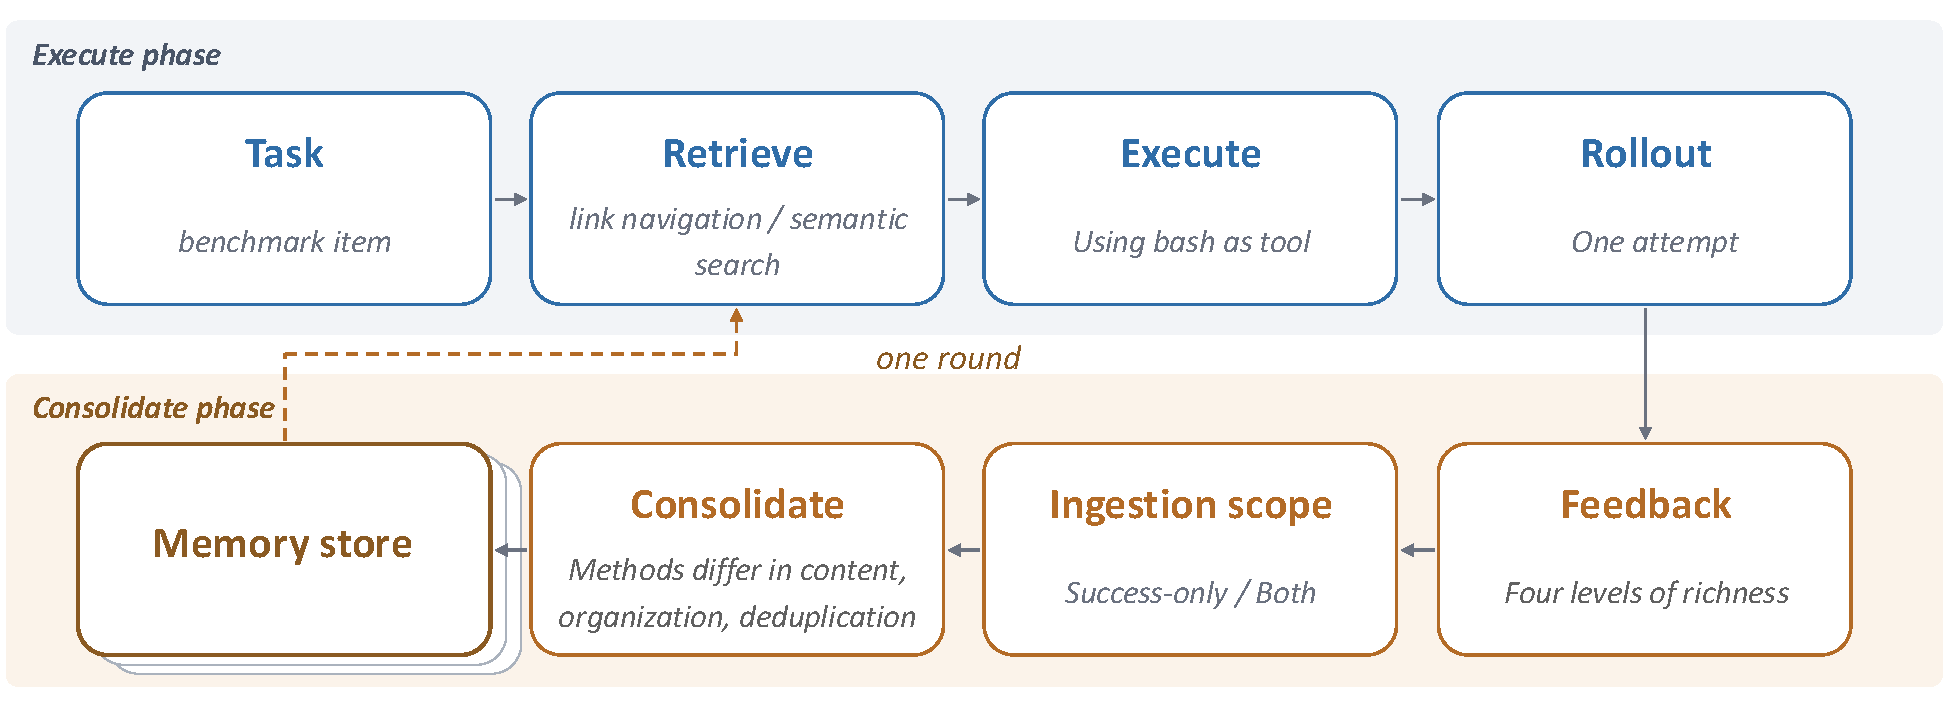
\includegraphics[height=4.5cm,width=\linewidth,keepaspectratio]{fig_overview_full.pdf}
  \caption{Procedural memory consolidation workflow.}
  \label{fig:overview-workflow}
\end{subfigure}%
\hfill%
\begin{subfigure}[b]{0.43\linewidth}
  \centering
  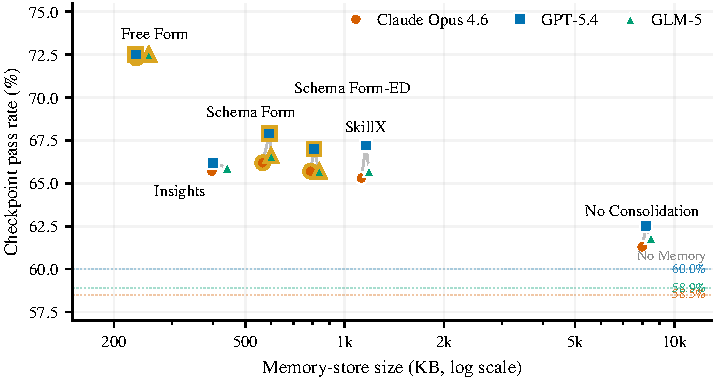
\includegraphics[height=4.5cm,width=\linewidth,keepaspectratio]{fig_filter.pdf}
  \caption{Memory-store size vs.\ checkpoint pass rate.}
  \label{fig:filter-size}
\end{subfigure}
\caption{\textbf{Workflow and key results.}
(a)~The multi-round loop enables continual learning by consolidate agent execution traces and feedback into reusable procedural memory.
(b)~Memory-store size and checkpoint performance across consolidation methods
and model variants. \method achieves higher checkpoint pass rate with smaller memory store size.}
\label{fig:combined}
\end{figure}


Formally, this process is a multi-round execution--consolidation cycle (Figure~\ref{fig:overview-workflow}). During
the execution phase, given a task, the agent retrieves zero or more relevant
memory pages, acts on the environment through its tools, and records its actions
and observations as a raw rollout trace. An evaluator or human then provides
feedback based on the resulting environment state. During the consolidation
phase, a method reads the current store alongside eligible traces and feedback,
and abstracts them into reusable procedural knowledge: when a procedure
applies, which actions to perform, what failures may arise, and how to diagnose
and resolve them. The method then writes or merges this knowledge according to
the memory system's representation and interaction interface. One execution
pass followed by consolidation forms a round; only the updated memory store
carries into the next round, while the model parameters and harness remain
fixed.

Agent memory is a rapidly expanding design space, with new representations,
extraction rules, retrieval mechanisms, and update procedures appearing
continuously
\citep{memsurvey,selfevolving,amem,reasoningbank,insights,skillx}. Choosing
among overwhelming candidates resembles a classic Secretary Problem
\citep{ferguson1989secretary} with no known stopping rule, and exhaustive
evaluation is infeasible. Practitioners instead need higher-level principles
explaining which design dimensions matter, where human and system effort
produces the greatest return, and which interventions merely add constraints or
volume. We organize our study around three questions: \emph{(1) How should execution experience be consolidated into reusable
procedural memory? (2) Which feedback, trace ingestion scope, and refinement
choices most improve future execution? (3) Where should human effort be spent:
prescribing knowledge organization upfront or diagnosing failures reactively?}

Through controlled experiments and qualitative analysis, we derive actionable
answers to these questions. Our contributions are threefold:

\begin{itemize}[leftmargin=*,itemsep=2pt,topsep=3pt]
    \item \textit{Nimble but Effective Consolidation Method.} We introduce
    \(\mathcal{W}\)iki-based \(\mathcal{A}\)gent-\(\mathcal{S}\)ynthesized \(\mathcal{P}\)rocedural \(\mathcal{M}\)emory (\method), an agentic
    procedural-memory organizer for training-free continual learning. It
    consolidates agent execution traces and human feedback into persistent,
    interlinked wiki pages, achieving both the most compact knowledge store and
    the strongest downstream task performance among all compared methods
    (Figure~\ref{fig:filter-size}).
    \item \textit{Controlled Study.} To determine what makes procedural-memory
    consolidation effective, we systematically vary consolidation method,
    feedback type, trace-ingestion scope, and refinement rounds across three
    models, identifying which interventions most improve future execution.
    \item \textit{Learnings From a Bitter Lesson.} We distill our findings into
    a design principle: build a general-purpose memory
    system, but let the agent self-organize its procedural knowledge. Imposing
    domain-specific structure on procedural knowledge at design time harms
    performance. Instead, human intervention is most effective when applied
    reactively---through failure diagnosis, targeted feedback, and iterative
    refinement.
\end{itemize}
